\chapter{Preparation}
\label{chap:preparation}
\indent \indent
This chapter discusses the preparatory work done before beginning the project's implementation. §\ref{sec:preliminaries} introduces the relevant concepts, terminologies, and notations from cryptography, graphics, and unsupervised machine learning fundamental to the project, §\ref{sec:projectStrategy} discusses the methodologies used when approaching the design of the project's implementation, and §\ref{sec:startingPoint} provides an overview of the project's foundations.
\section{Preliminaries}
\label{sec:preliminaries}
\subsection{Homomorphic Encryption}
\label{sec:homomorphicEncryption}
\subsubsection{Introduction}
\indent \indent
There are two broad categories of cryptographic encryption schemes: private-key (symmetric) and public-key (asymmetric). While both can be applied to HE, this dissertation will address public-key encryption because it is the technique adopted by all HE schemes used in the project.
\smallskip \\ \indent
A public-key encryption scheme is defined by a triple of functions $\Pi = (\texttt{KeyGen}, \texttt{Enc}, \texttt{Dec})$. \texttt{KeyGen} is a function used to generate a \textit{public key} (\texttt{PK}) and \textit{private key}\footnote{The \textit{private key} is referred to as a \textit{secret key} by some literature. While these terms are equivalent, general convention is to use \textit{secret key} in relation to symmetric encryption, and \textit{private key} when discussing asymmetric.} (\texttt{SK}) such that $(\texttt{PK}, \texttt{SK}) \leftarrow \texttt{KeyGen}(1^l)$, where the security parameter, $l$, measures how hard it is for an adversary to break the scheme\footnote{An $l$-bit security parameter would require an expected $2^l$ attempts to guess the keys.}. Denoting the space of all possible plaintext messages as $\mathcal{M}$ and ciphertext messages as $\mathcal{C}$, a message $m \in \mathcal{M}$ is encrypted into its corresponding ciphertext $c \in \mathcal{C}$ by $c \leftarrow \texttt{Enc}_\texttt{PK}(m)$. Similarly $c$ is decrypted back into $m$ by $m \leftarrow \texttt{Dec}_\texttt{SK}(c)$.
\smallskip \\ \indent
In order to extend $\Pi$ into a HE scheme, a fourth function $\texttt{Eval}(f, c_1, \ldots, c_n)$ must be introduced. The evaluation function, $\texttt{Eval}$ applies a Boolean circuit, $f$, to the ciphertext arguments, $c_1, \ldots, c_n$ such that, for all arguments, it holds that
\begin{equation}
    \texttt{Dec}_\texttt{SK}(\texttt{Eval}(f, c_1, \ldots, c_n)) = f(m_1, \ldots, m_n)
\end{equation}
where $m_1, \ldots, m_n$ are the plaintext equivalents of $c_1, \ldots, c_n$. This is, perhaps, better illustrated by Figure \ref{fig:homomorphicEncryption} below.
\begin{figure}[ht]
    \centering
    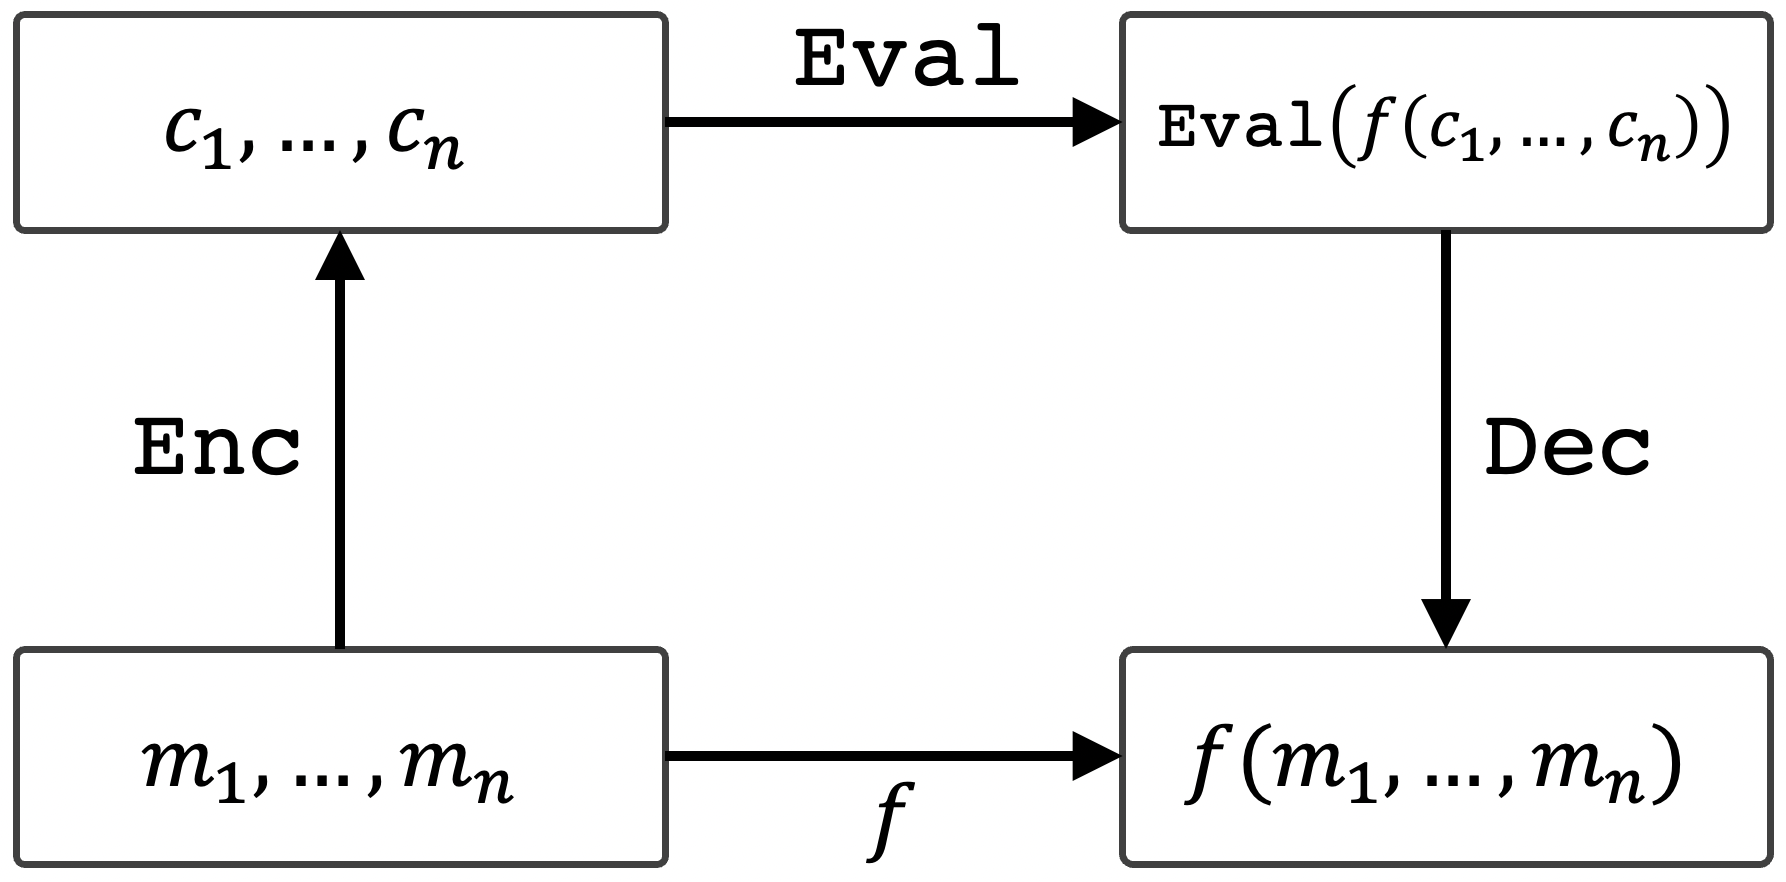
\includegraphics[width=0.5\textwidth]{figures/homomorphicEncryption.png}
    \caption[Homomorphic Encryption]{Homomorphic Encryption}
    \label{fig:homomorphicEncryption}
\end{figure}
Theoretically, a \textit{fully} homomorphic scheme\footnote{The prefix \textit{fully} derives from the existence of \textit{partially} homomorphic schemes. A partially homomorphic scheme will only allow certain operations on the ciphertext - usually multiplication and division - and have existed for many years. Some examples of partially homomorphic schemes include RSA, ElGamal, and Paillier encryption ~\cite{PartialSchemes}.} allows the evaluation of Boolean circuits indefinitely. However, in practice, the time complexity of operations means many schemes are \textit{levelled} homomorphic schemes. This means they only support operations up to a \textit{bounded depth} - that is, only a predefined number of circuits can be applied to a ciphertext before the plaintext becomes irrecoverable. The maximum depth is a critical factor when applying HE to practical problems because it significantly limits the scope of supported algorithms.
\subsubsection{Ring Learning with Errors}
\indent \indent
For an encryption scheme to be \textit{perfectly secure}, a ciphertext must provide no additional information about its plaintext (see Equation \ref{eq:def1}). In other words, the probability of generating a given ciphertext from a particular plaintext is independent of the plaintext (see Equation \ref{eq:def2}). The two equations below can be shown to be equivalent using Bayes' rule. 
\begin{equation}
    \label{eq:def1}
    \probP(M = m \: | \: C = c) = \probP(C = c)
\end{equation}
\begin{equation}
    \label{eq:def2}
    \probP(C = c \: | \: M = m) = \probP(M = m)
\end{equation}
for all $m \in \mathcal{M}$, $c \in \mathcal{C}$.
\smallskip \\ \indent
While it is possible to create perfectly secure encryption schemes\footnote{For example, the One-Time Pad[OTP]}, they are impractical in real applications. Therefore, \textit{computational security} is considered sufficient. Relying on the hardness of certain mathematical problems, computational security means that an encryption scheme is \textit{practically unbreakable}: the most efficient known algorithm for breaking a cipher would require more computational steps than an attacker with unlimited hardware could perform. For example, the RSA encryption scheme relies on the fact that there exists no known, efficient algorithm for computing the prime factors of a large number on a classical computer - the integer factorisation problem. In complexity theory, this problem falls into the set of $\mathcal{NP}$.
\smallskip \\ \indent
Similarly, the HE schemes used in this project rely upon computational security. They utilise the hardness of the \textit{ring learning with errors} (henceforth RLWE) problem introduced by Lyubashevsky et al.\ ~\cite{RLWE}. A polynomial-time reduction from the \textit{shortest vector problem} to RLWE can be derived. Therefore, since the shortest vector problem is $\mathcal{NP}$-hard under the correct choice of parameters, it is safe to rely upon RLWE for computational security.
\smallskip \\ \indent
To understand the RLWE problem, knowledge of group theory is required. The relevant definitions are introduced in Appendix \ref{app:groups}. The RLWE problem requires the ring formed by the set of polynomials modulo $\Phi (X)$ that also have coefficients in $\mathbb{Z}_q$\footnote{$\mathbb{Z}_q$ is the set of integers modulo $q$. For example, $\mathbb{Z}_7 = \{0, 1, 2, 3, 4, 5, 6\}$.}. Known as a \textit{quotient ring}, this can be denoted by $\mathcal{R}_q = \mathbb{Z}[X] / (\Phi(X))$, where $\Phi(X)$ is an \textit{irreducible polynomial} - a polynomial which cannot be factored into two non-constant polynomials.
\smallskip \\ \indent
Informally, RLWE describes the problem of finding an unknown $s \in \mathcal{R}_q$ given a polynomial vector computed using $s$ and some sampled errors. An encryption scheme can be created such that, after encoding a plaintext vector, $\vec{v}$, as a list of polynomials and it to a polynomial using a secret polynomial, it is infeasible to recover $\vec{v}$ in polynomial time.
\smallskip \\ \indent
The HE schemes discussed in this dissertation rely upon the RLWE problem to assert \textit{indistinguishable encryptions under a chosen-plaintext attack} (IND-CPA) security. Fundamentally, any encryption scheme is IND-CPA secure if, when attacked by a probabilistic, polynomial-time adversary, the chances of correctly deciding which of two plaintexts a particular ciphertext corresponds to is even. Therefore, in practice, even if an adversary has access to an encryption \textit{oracle}, the adversary's chances of calculating the correct plaintext when given a ciphertext should be no better than if they were randomly guessing. 
\smallskip \\ \indent
Practically, HE schemes choose a \textit{cyclotonic polynomial} for $\Phi(X)$, where the $n$-th cyclotonic polynomial, $\Phi_n(X)$, is defined as
\begin{equation}
    \Phi_n(X) = \prod_{k \in [1, n]; \; gcd(k, n = 1)} X - e^\frac{2 i \pi k}{n}
\end{equation}
In order to speed up computation, $n$ is selected to be an even power of two. Consequently, $\Phi_n(X) = X^\frac{n}{2} + 1$. This allows the \textit{number theoretic transform} (NTT)\footnote{A specialisation of the discrete Fourier transform, the NTT is a generalisation of the Fast Fourier transform in the case of finite fields. ~\cite{NTT}}. The advantage of this is that it can be easily accelerated using hardware ~\cite{Hardware}.
\smallskip \\ \indent
The sampled errors used when deriving ciphertexts imply almost exponential error growth in the number of multiplications applied. The limited depth property of levelled HE schemes directly results from this. However, the relative growth size can be reduced by increasing the modulus $q$. Although, if a polynomial degree of size $n/2$ is used, efficient attacks exist against the RLWE problem for a small value of $q$ ~\cite{HEStandard}. Therefore, a fundamental trade-off is introduced between the supported depth of multiplication and the security level.





\subsection{Moving Object Detection}
\label{sec:movingObjectDetection}
\subsubsection{Introduction}
\indent \indent
\textit{Image segmentation} is a well-established problem in the fields of digital image processing and computer vision research. The problem describes the process of partitioning a digital image into multiple regions, represented as sets of pixels. The goal is to simplify an image representation so that it is easier to, for example, locate objects or boundaries, allowing further analysis. More precisely, image segmentation describes labelling each pixel of an image such that all pixels sharing a particular characteristic are assigned the same label ~\cite{Shapiro}.
\smallskip \\ \indent
There are two broad categories of segmentation techniques: \textit{semantic} \cite{Semantic} and \textit{instance} \cite{Instance}. This dissertation will focus on semantic segmentation through moving object detection because videos will be segmented into two categories: foreground and background, rather than labelling individual instances of objects.
\smallskip \\ \indent
To perform \textit{foreground extraction}, also known as \textit{background subtraction}, the background of an image must be modelled so that changes in the scene can be detected. This is an unsolved problem. Image data can be very diverse, with variable lighting and repetitive movements (like leaves and shadows) making robust models hard to develop.
\smallskip \\ \indent
Once a background model has been developed, it can be used to detect moving objects in videos by comparing each frame to a reference frame and extracting the differences. There are several methods for achieving this. Below are five algorithms investigated for this dissertation.
\subsubsection{Frame Differencing}
\indent \indent
\textit{Frame differencing} is the most straightforward background subtraction algorithm ~\cite{FrameDifferencing}. First, a reference frame is established. There are several options for this, including selecting the first frame, or continually updating to the frame previously received. Challenges include ensuring the model can adapt to permanent changes, like a fence being added to a property, and accounting for random noise. Updating the reference too frequently can cause issues with slow-moving objects becoming occluded.
\smallskip \\ \indent
Once the reference frame, $B$, has been selected, the foreground can be extracted. Denoting each frame at time $t$ as $f_t$, the value of each pixel in $B$, $P(B)$, can be subtracted from the corresponding pixel in $f_t$, $P(f_t)$. The mathematical definition is given by Equation\ref{eq:frameDifferencing}.
\begin{equation}
    \label{eq:frameDifferencing}
    P(F_t) = P(f_t) - P(B)
\end{equation}
where $F$ represents the frames in the resultant video.
\subsubsection{Mean Filter}
\indent \indent
A \textit{mean filter} approach to moving object detection attempts to overcome the weaknesses of frame differencing in selecting a reference frame ~\cite{MeanFilter}. Instead of taking a frame directly from the video, the value of $B$ at time $t$ is calculated using Equation \ref{eq:meanFilter}.
\begin{equation}
    \label{eq:meanFilter}
    B = \frac{1}{N} \sum^N_{i=1} f_{t-i}
\end{equation}
where $N$ is the number of preceding images included in the average, and $f_t$ is the frame in the video at time $t$. $N$ would depend on the video speed and the amount of motion expected in the video.
\smallskip \\ \indent
After $B$ has been calculated at time $t$, the value of the resultant video $F_t$ can be calculated using the same method as frame differencing, given by Equation \ref{eq:frameDifferencing}.
\subsubsection{Median Filter}
\indent \indent
The \textit{median filter} algorithm is similar to performing mean filter extraction. Instead of using the mean to calculate the reference frame, the median of the preceding $N$ frames is used ~\cite{MeanFilter}. Then, the moving objects are extracted by subtracting the reference frame from each frame in the video, according to Equation \ref{eq:frameDifferencing}.
\subsubsection{Gaussian Average}
\label{sec:gaussianAverage}
\indent \indent
Wren et al.\ originally proposed fitting a Gaussian probabilistic density function to the most recent $N$ frames ~\cite{Wren}. Rather than storing an image as the reference frame, this method stores a mean and variance for each pixel. When a new frame is received, the likelihood of each pixel is calculated. Assuming that the background is the most common value for a pixel, the foreground can be segmented by grouping the pixels with a sufficiently low likelihood.
\smallskip \\ \indent
Rather than recalculating the mean every time a frame is received - giving an $O(n^2)$ time complexity - the algorithm can be implemented using cumulative functions for the mean and variance to achieve a linear time complexity. The functions are defined by Equation \ref{eq:mean} and Equation \ref{eq:variance} respectively. 
\begin{equation}
    \label{eq:mean}
    \mu_t =
    \begin{cases}
        f_0 & \text{if $t = 0$} \\
        \alpha f_t + (1 - \alpha) \mu_{t-1} & \text{otherwise}
    \end{cases}
\end{equation}
\begin{equation}
    \label{eq:variance}
    \sigma^2_t =
    \begin{cases}
        c & \text{if $t = 0$} \\
        d^2 \alpha + (1 - \alpha) \sigma^2_{t-1} & \text{otherwise}
    \end{cases}
\end{equation}
where $\alpha$ determines the size of the \textit{temporal window} used to fit the Gaussian model\footnote{$\alpha$ weights frames according to age. Eventually, an old frame will be weighted so insignificantly that its impact is negligible. Therefore, it determines how far into the past the model uses to predict future pixels.}, $d = |f_t - \mu_t|$ gives the Euclidean distance from the pixel to the mean, and $c$ is some constant defined by the model creator. 
\smallskip \\ \indent
From these models, the foreground can be extracted according to Equation \ref{eq:meanThreshold},
\begin{equation}
    \label{eq:meanThreshold}
    \frac{|f_t - \mu_t|}{\sigma_t} > k
\end{equation}
where $k$ is a constant that the model creator can tune to achieve optimal results.
\smallskip \\ \indent
A variant of this algorithm might only update the model if a pixel is believed to be in the background. This prevents the model from becoming skewed if there is lots of movement. However, it requires the entire frame to be initially background and struggles to cope with constant changes.
\subsubsection{Gaussian Mixture Models}
\indent \indent
Stauffer and Grimson proposed \textit{Gaussian mixture models} (henceforth GMMs) for moving object detection in 1999 ~\cite{Stauffer}. GMMs are probabilistic models that represent the presence of normally distributed subpopulations within an overall population. They are particularly useful because they don't require the subpopulation of a data point to be identified. Instead, subpopulations are labelled automatically, constituting \textit{unsupervised machine learning}.
\smallskip \\ \indent
There are two types of parameters necessary for GMMs, the \textit{component weights}, and the component \textit{means} and \textit{variances}. For a GMM with $N$ components, the $i^\text{th}$ component has $\mu_i$ and variance $\sigma_i$ in the \textit{univariate case}, and mean $\vec{\mu}_i$ and a covariance matrix $\Sigma_i$ in the \textit{multivariate case}. The component weights, $\phi_k$ for component $k$, are constrained by the equation $\sum^K_{i=1} \phi_i = 1$. If the component weights aren't learned, they are known as an \textit{a-priori}\footnote{A probability derived purely through deductive reasoning.} distribution over components such that $\probP(x \text{ generated by component k}) = \phi_k$. If the component weights are learned, they are known as \textit{a-posteriori}\footnote{From Bayesian statistics, referring to conditional probability $\probP(A | B)$.} estimates of the component probabilities given the data.
\smallskip \\ \indent
When fitting a GMM, the Gaussian distributions are tuned to match the distributions observed in the data. A common method for this is to use \textit{expectation maximisation} (EM), if the number of components is known. If all of the data is available, it can be incorporated into this stage to achieve the most accurate fitting. However, only a subset of the data will likely be available in practice, so the GMM will extrapolate to more values. This technique can also be taken advantage of if there is limited time to perform fitting.
\smallskip \\ \indent
Once a GMM has been fitted, it can be used for inference. This dissertation will focus on inference for \textit{clustering} because it is most useful for moving object detection. The posterior component assignment probabilities can be estimated using Bayes' theorem over the GMM parameters. Knowing the component that a data point most likely belongs to provides a way to group the points into clusters. In the scenario of moving object detection, this would be two clusters: the foreground and the background.






\section{Project Strategy}
\label{sec:projectStrategy}
\subsection{Requirements Analysis}
\label{sec:requirements}
\indent \indent
The requirements for this project are listed below. The project required the development of theoretical knowledge before implementation began so the requirements evolved as understanding matured. The original requirements are given in Appendix \ref{app:proposal} for comparison. The requirements have been grouped into two categories. The first, labelled $A$, are the core requirements essential to the project's success. The second, labelled $B$, are extensions, aiming to improve understanding or further the investigation into HE and surveillance.
\begin{table}[h!]
    \centering
    % \resizebox{\textwidth}{!}{%
    \begin{tabular}{|>{\centering\arraybackslash}m{0.5cm}||m{10.9cm}|>{\centering\arraybackslash}m{1.63cm}|>{\centering\arraybackslash}m{1.91cm}|}
        \hline
        & \textrm{\textbf{Requirement}} & \textrm{\textbf{Priority}} & \textrm{\textbf{Difficulty}} \\
        \hline \hline
        \texttt{A1} & \textrm{Implement a client-server application allowing videos to be homomorphically encrypted and transmitted in both directions.} & \color{Red}\textrm{High} & \color{Dandelion}\textrm{Medium} \\
        \hline
        \texttt{A2} & \textrm{Implement background subtraction models that can extract moving objects from homomorphically encrypted videos.} & \color{Red}\textrm{High} & \color{Dandelion}\textrm{Medium} \\
        \hline
        \texttt{A3} & \textrm{Evaluate the accuracy of HE inference to investigate its applicability to real systems.} & \color{Red}\textrm{High} & \color{Green}\textrm{Low} \\
        \hline \hline
        \texttt{B1} & \textrm{Implement a bespoke HE scheme and integrate it into the core application, providing the same functionality as the established scheme already used.} & \color{Dandelion}\textrm{Medium} & \color{Red}\textrm{High} \\
        \hline
        \texttt{B2} & \textrm{Analyse the security of the encryption schemes used in the project.} & \color{Green}\textrm{Low} & \color{Red}\textrm{High} \\
        \hline
        \texttt{B3} & \textrm{Implement a deep-learning object recognition algorithm acting on HE data following Cryptonets \cite{Dowlin}.} & \color{Green}\textrm{Low} & \color{Red}\textrm{High} \\
        \hline
    \end{tabular}%}
    \caption[Requirements Analysis]{Requirements analysis.}
\end{table}
\subsection{Methodology}
\indent \indent
Different stages of the project were best suited to different development methodologies. For core components, a waterfall methodology was adopted ~\cite{Waterfall}. The requirements were detailed and unambiguous, so the project lent itself to a structured methodology, not requiring the flexibility of an iterative approach. The model's stages are detailed below.
\smallskip \\ \indent
The results of the \textit{requirements analysis} stage have been provided in §\ref{sec:requirements}. This stage is where most of the research was performed to ensure the project's design was better informed.
\smallskip \\ \indent
The \textit{design} phase incorporates expanding on the requirements into a physical project; this includes, for example, creating the class diagrams shown in Figure \ref{fig:clientUML}, Figure \ref{fig:serverUML}, and Figure \ref{fig:mekksUML}.
\smallskip \\ \indent
The \textit{implementation} and \textit{testing} stages were intertwined where possible in order to promote a test-driven approach to development. This was made easier by the object-oriented methodology and unit testing practices adopted.
\smallskip \\ \indent
The \textit{evaluation} stage replaces the \textit{maintenance} stage of the traditional Waterfall model. This stage involves running experiments to evaluate the project. 
\smallskip \\ \indent
When working on extensions, an iterative model was more appropriate. The main reason for this was that less time had been dedicated to researching these components, so implementation was riskier. Consequently, a rapid cyclical development model requiring components to be decomposed would allow any problems to be discovered sooner, limiting impact. Therefore, the Agile model, depicted in Figure \ref{fig:agile} was selected. Regular supervisor meetings allowed Agile's sprint system to be utilised so that a project prototype could be presented in each meeting to ensure thorough progression tracking.
\begin{figure}[h!]
    \centering
    \begin{subfigure}[b]{0.495\textwidth}
        \centering
        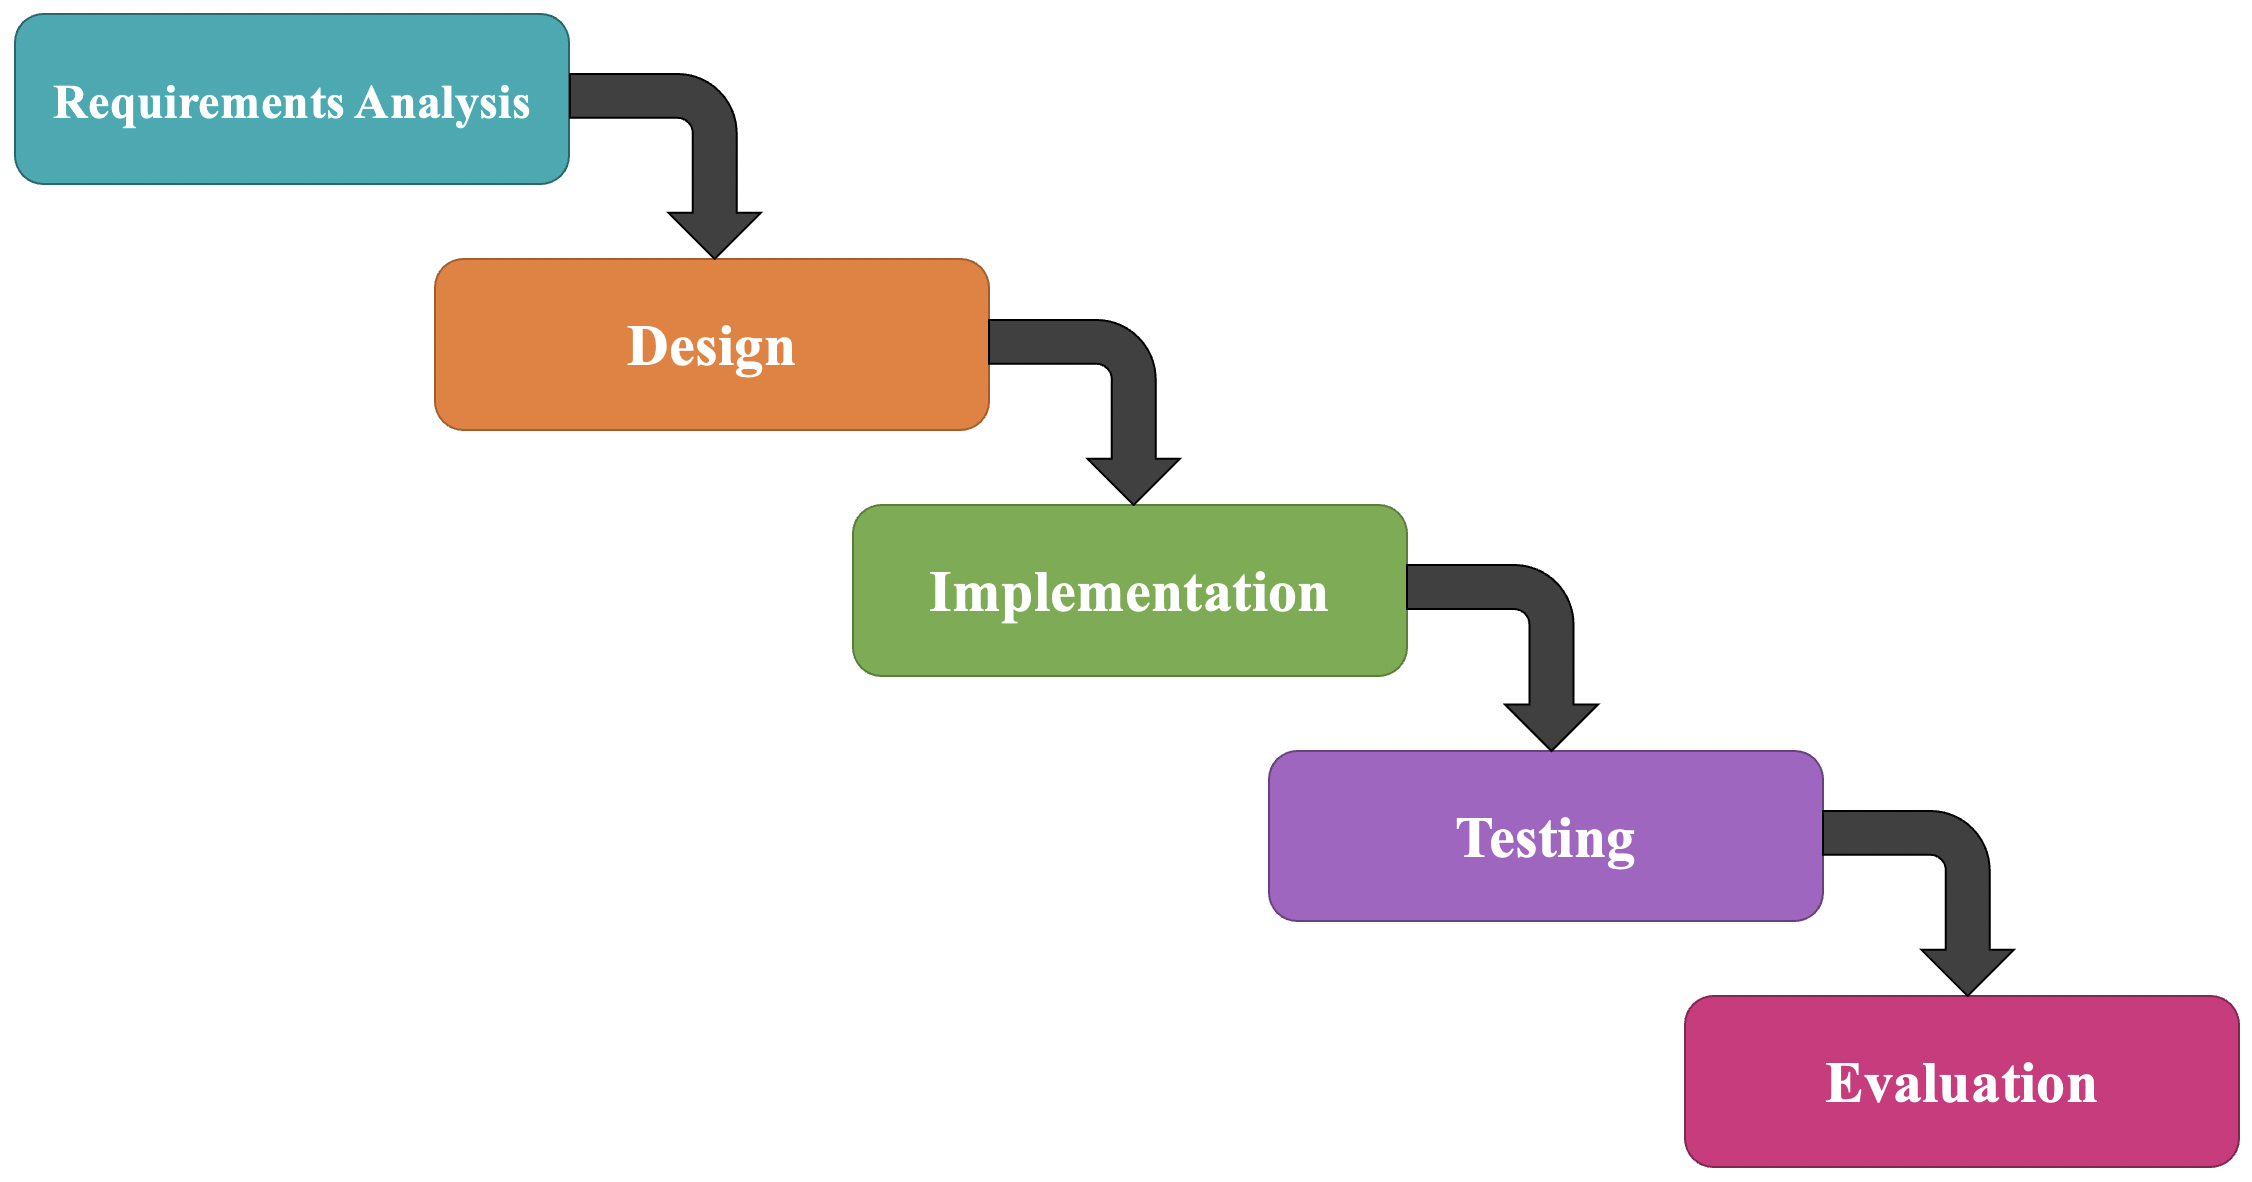
\includegraphics[width=1.1\textwidth]{figures/waterfall.png}
        \caption{The Waterfall Development Model}
        \label{fig:waterfall}
    \end{subfigure}
    \hfill
    \begin{subfigure}[b]{0.495\textwidth}
        \centering
        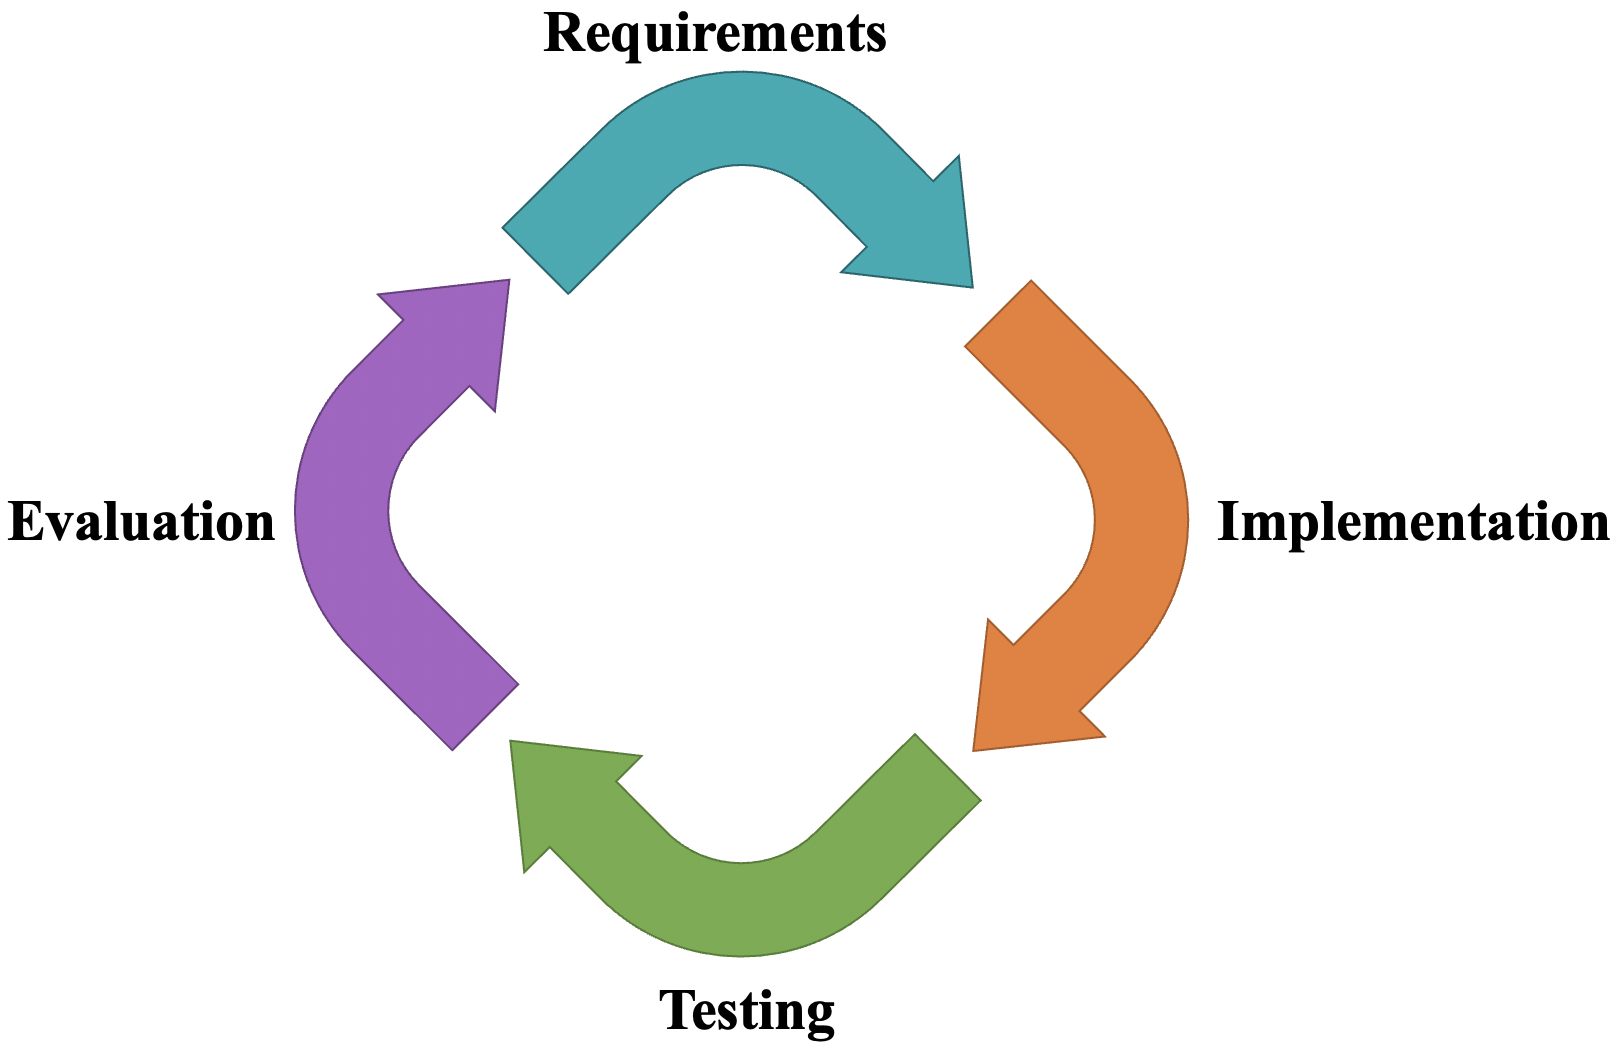
\includegraphics[width=0.9\textwidth]{figures/agile.png}
        \caption{The Agile Development Model}
        \label{fig:agile}
    \end{subfigure}
    \caption{Development Models}
\end{figure}
\begin{figure}[h!]
    \centering
    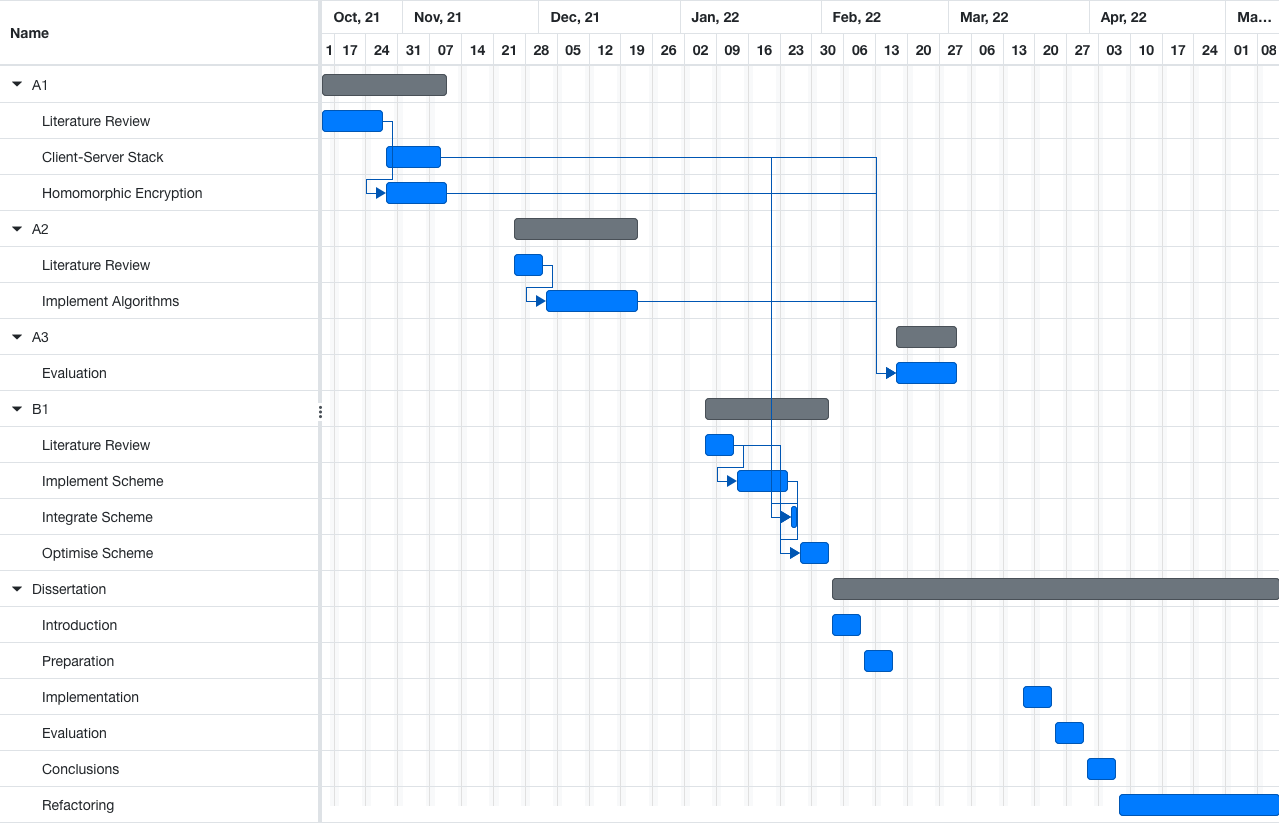
\includegraphics[width=\textwidth]{figures/gantt.png}
    \caption{Project Timeline}
    \label{fig:gantt}
\end{figure}
\smallskip \\ \indent
A Gantt chart of the project's timeline is shown in Figure \ref{fig:gantt}.
\subsection{Testing}
\label{sec:testing}
\indent \indent
Unlike traditional software engineering, machine learning does not provide precise criteria against which correctness can be verified. The models used for background subtraction are probabilistic, so the outputs cannot be precisely predicted.  Consequently, a variety of testing methodologies were required.
\subsubsection{Unit Tests}
\indent \indent
Designed for testing atomic units of source code, unit testing utilises the independence resulting from the object-oriented design approach to test components in isolation. Test cases provide expected, boundary, and erroneous data to ensure function results match the expected. Unit tests can be automated to allow repeated checks as changes to the source code are made, ensuring errors aren't introduced.
\smallskip \\ \indent
Unit tests were particularly useful when completing the first extension for verifying the correctness of the encoding, encryption, and decryption functions and the HE Boolean circuits.
\subsubsection{Integration Tests}
\indent \indent
Integration tests increase the scope of functionality covered by each test by ensuring separate modules interact correctly. Once unit testing has been completed, these tests aggregate verified modules and provide data to ensure the output is correct.
\smallskip \\ \indent
Integration testing was useful in verifying that the software stack functioned correctly. For example, ensuring the client and server communicated correctly. While some integration testing can be automated, more complex engineering work was prioritised over creating a comprehensive testing suite, so manual integration testing was primarily used.
\subsubsection{Manual Verification}
\indent \indent
Manual verification was used to overcome the challenges of testing the background subtraction models. Since the project involves video data, human inspection provides a good intuition of whether or not a background has been correctly removed. If a more detailed analysis is required, pixel values can be compared to check for expected results or verify consistency across multiple tests.






\section{Starting Point}
\label{sec:startingPoint}
\subsection{Knowledge and Experience}
\indent \indent
Prior to beginning the project, the following relevant Tripos courses had been completed: \textit{Scientific Computing}, \textit{Machine Learning and Real-world Data}, \textit{Software and Security Engineering}, \textit{Concurrent and Distributed Systems}, \textit{Data Science}, \textit{Computer Networking}, and \textit{Security}. The Part II course, \textit{Cryptography} was also useful in understanding the theoretical underpinnings of encryption.
\smallskip \\ \indent
However, it should be noted that HE is not included in the scope of the Cryptography course, so theory was learned independently of Tripos studies. The study of applied HE is sparsely documented, so most understanding came from academic papers; notably \cite{CKKS} and \cite{SEAL}. Although, articles such as \cite{BrilliantHE} were more useful for foundational knowledge.
\smallskip \\ \indent
Similarly, there was little mention of computer vision artificial intelligence in Tripos, so most understanding came from independent research. Academic papers such as \cite{Stauffer} and \cite{Kulchandani} were helpful, particularly when considering privacy-preserving computer vision. Some understanding also came during a summer internship completed in the field of object recognition deep learning.
\subsection{Tools Used}
\subsubsection{Programming Languages}
\indent \indent
All code written for this dissertation was written in \textit{Python} ~\cite{Python}. The main reasons for this were the large machine learning ecosystem, ease of use, and ease of debugging. These factors allowed for quick implementation, making Python best suited to the project's tight schedule. 
\smallskip \\ \indent
However, Python is not a language traditionally used for cryptographic applications. Usually, lower-level, faster languages like C++ are favoured. Since the focus of the project was investigating the efficacy of moving object detection in the HE domain, the speed of execution was not prioritised over the speed of implementation.
\subsubsection{Software Development}
\indent \indent
\textit{Visual Studio Code} \cite{VSCode} development environment was used for writing code because of support for Python as well as a wide variety of plugins that allow integration of other valuable tools such as ESLint.  In addition, \textit{Git} \cite{Git} and \textit{GitHub} \cite{Github} were used for version control and source code management. \textit{OneDrive} \cite{OneDrive} was also used to hold another backup for safety.
\subsubsection{Encryption Schemes}
\indent \indent
The project focuses on HE schemes based on the RLWE problem. The main reason for this was the availability of academic literature discussing them. In particular, the CKK scheme \cite{CKKS} was selected because it supports representing real numbers\footnote{Versus the BFV scheme, which only supports integers ~\cite{BFV1, BFV2}.}. However, the project is designed to allow any HE scheme following the same API to be substituted in CKKS's place.
\subsubsection{Libraries}
\indent \indent
The project uses Microsoft's SEAL library \cite{SEAL}, which provides a C++ implementation of the CKKS scheme. This was chosen because of the extensive optimisations that have been applied. In particular, SEAL uses a residue-number-system variant of CKKS to support large plaintext moduli. SEAL was integrated using a Python wrapper library ~\cite{Wrapper}.
\subsubsection{Datasets}
\indent \indent
There were two publicly available datasets used in this project:
\begin{itemize}
    \item The Moving-MNIST dataset contains ten thousand sequences of length twenty frames showing two handwritten digits from the standard MNIST dataset moving in a $64 \times 64$ pixel frame ~\cite{MovingMNIST, MNIST}. This is a relatively simple dataset to perform moving object detection on because it only contains white objects on a black background. Therefore, it was useful in providing a baseline for the performance of the inference algorithms.
    \item The LASIESTA dataset contains sequences showing individuals moving across static backgrounds ~\cite{LASIESTA}. Specifically designed to evaluate segmentation algorithms, this dataset provides more realistic examples of surveillance footage so allows a truer evaluation of moving object detection in the HE domain.
\end{itemize}
\subsubsection{Licensing}
\indent \indent
All software dependencies in this project use permissive libraries that allow their code to be used without restrictions. The same is true for the datasets. Table \ref{tab:licensing} gives the specific licenses.
\begin{table}[h!]
\centering
\resizebox{0.5\textwidth}{!}{%
\begin{tabular}{|p{4cm}|p{4cm}|}
    \hline
    \textrm{\textbf{Dependency}} & \textrm{\textbf{Licence}} \\
    \hline \hline
    \texttt{Multiprocessing} & \multirow{3}{*}{\textrm{3-Clause BSD ~\cite{BSD}}} \\ 
    \texttt{NumPy} & \\ 
    \texttt{SymPy} & \\
    \hline
    \texttt{Microsoft SEAL} & \multirow{3}{*}{\textrm{MIT ~\cite{MIT}}} \\
    \texttt{SEAL-Python} & \\
    \texttt{PyJoules} & \\
    \hline
    \texttt{Matplotlib} & \multirow{3}{*}{\textrm{PSFL ~\cite{PSFL}}} \\ 
    \texttt{Python} & \\
    \texttt{Tkinter} & \\
    \hline
\end{tabular}}
\caption{Licenses}
\label{tab:licensing}
\end{table}
\subsection{Computer Resources}
\indent \indent
The original project proposal mentioned that external computational resources might have been required during the implementation phase, such as AWS or Microsoft Azure. However, the project was entirely developed, tested, and evaluated on a MacBook Pro laptop. The specifications are listed below, in Table \ref{tab:specs}.
\begin{table}[h!]
\centering
\begin{tabular}{>{\hspace{1em}}l l}
    \myheading{\textrm{Processor}}
    \textrm{CPU}                       & \SI{8}{\; Cores}                                            \\
    \textrm{GPU}                       & \SI{14}{\; Cores}                                           \\
    \textrm{Neural Engine}             & \SI{16}{\; Cores}                                           \\
    \textrm{Memory Bandwidth}          & \SI{200}{\; GB \per s}                                      \\
    \myheading{\textrm{Memory}}
    \textrm{RAM}                       & \SI{32}{\; GB \text{ (unified memory)}}                     \\
\end{tabular}
\caption{Computer Specifications}
\label{tab:specs}
\end{table}
